\section{Introduction}


Recent natural language generation systems have made remarkable progress in producing well-formed text, especially with massive pretrained language models.
Those models are typically trained using maximum likelihood estimation (MLE) with a large amount of data supervisions. 
Despite its successes, the standard training method suffers from limited applicability to many emerging text generation problems, where little or no supervised data is available. Prominent examples of such low-data problems include generating prompts to control the massive LMs~\citep{yin2019benchmarking,shin2020autoprompt,zhong2021meta,liu2021pre}, learning text generation from noisy or even negative data, generating adversarial text attacks for robustness study~\citep{wallace2019universal,atanasova2020generating}, and others (Figure~\ref{fig:first-figure}, right). Due to the failure of standard MLE, people have had to devise specialized algorithms for those problems respectively.

Reinforcement learning (RL)~\citep{sutton2018reinforcement} offers an alternative principled framework for learning from arbitrary reward functions.
However, RL by far has made limited success for training text generation, primarily due to the key challenges of \emph{sparse reward} (i.e., a single reward signal is received only after the whole text sequence is generated) and \emph{large action space} (i.e., a vocabulary of millions of words).
For instance, a popular family of RL algorithms studied extensively for text generation is the policy-based~\citep{williams1992simple} or actor-critic based~\citep{bahdanau2016actor,rennie2017self} algorithms, with policy gradient (PG) being the most prevalent example \citep{ranzato2015sequence,li2016deep,rennie2017self,tan2018connecting,pasunuru2018multi,paulus2018a}. Those algorithms train the model with \emph{on-policy} updates, i.e., the text samples used for estimating policy gradients are from the target model itself. Due to the exponentially large space of sequences, on-policy updates often suffer from extremely high variance and low data efficiency (e.g., most model samples are not useful for learning). Thus directly training with PG from scratch is usually impossible. In practice, the model has to be initialized by MLE training, followed by PG as finetuning, which often leads to limited improvement~\citep{Choshen2020On,wu2018study}.


\begin{figure*}
    \centering
    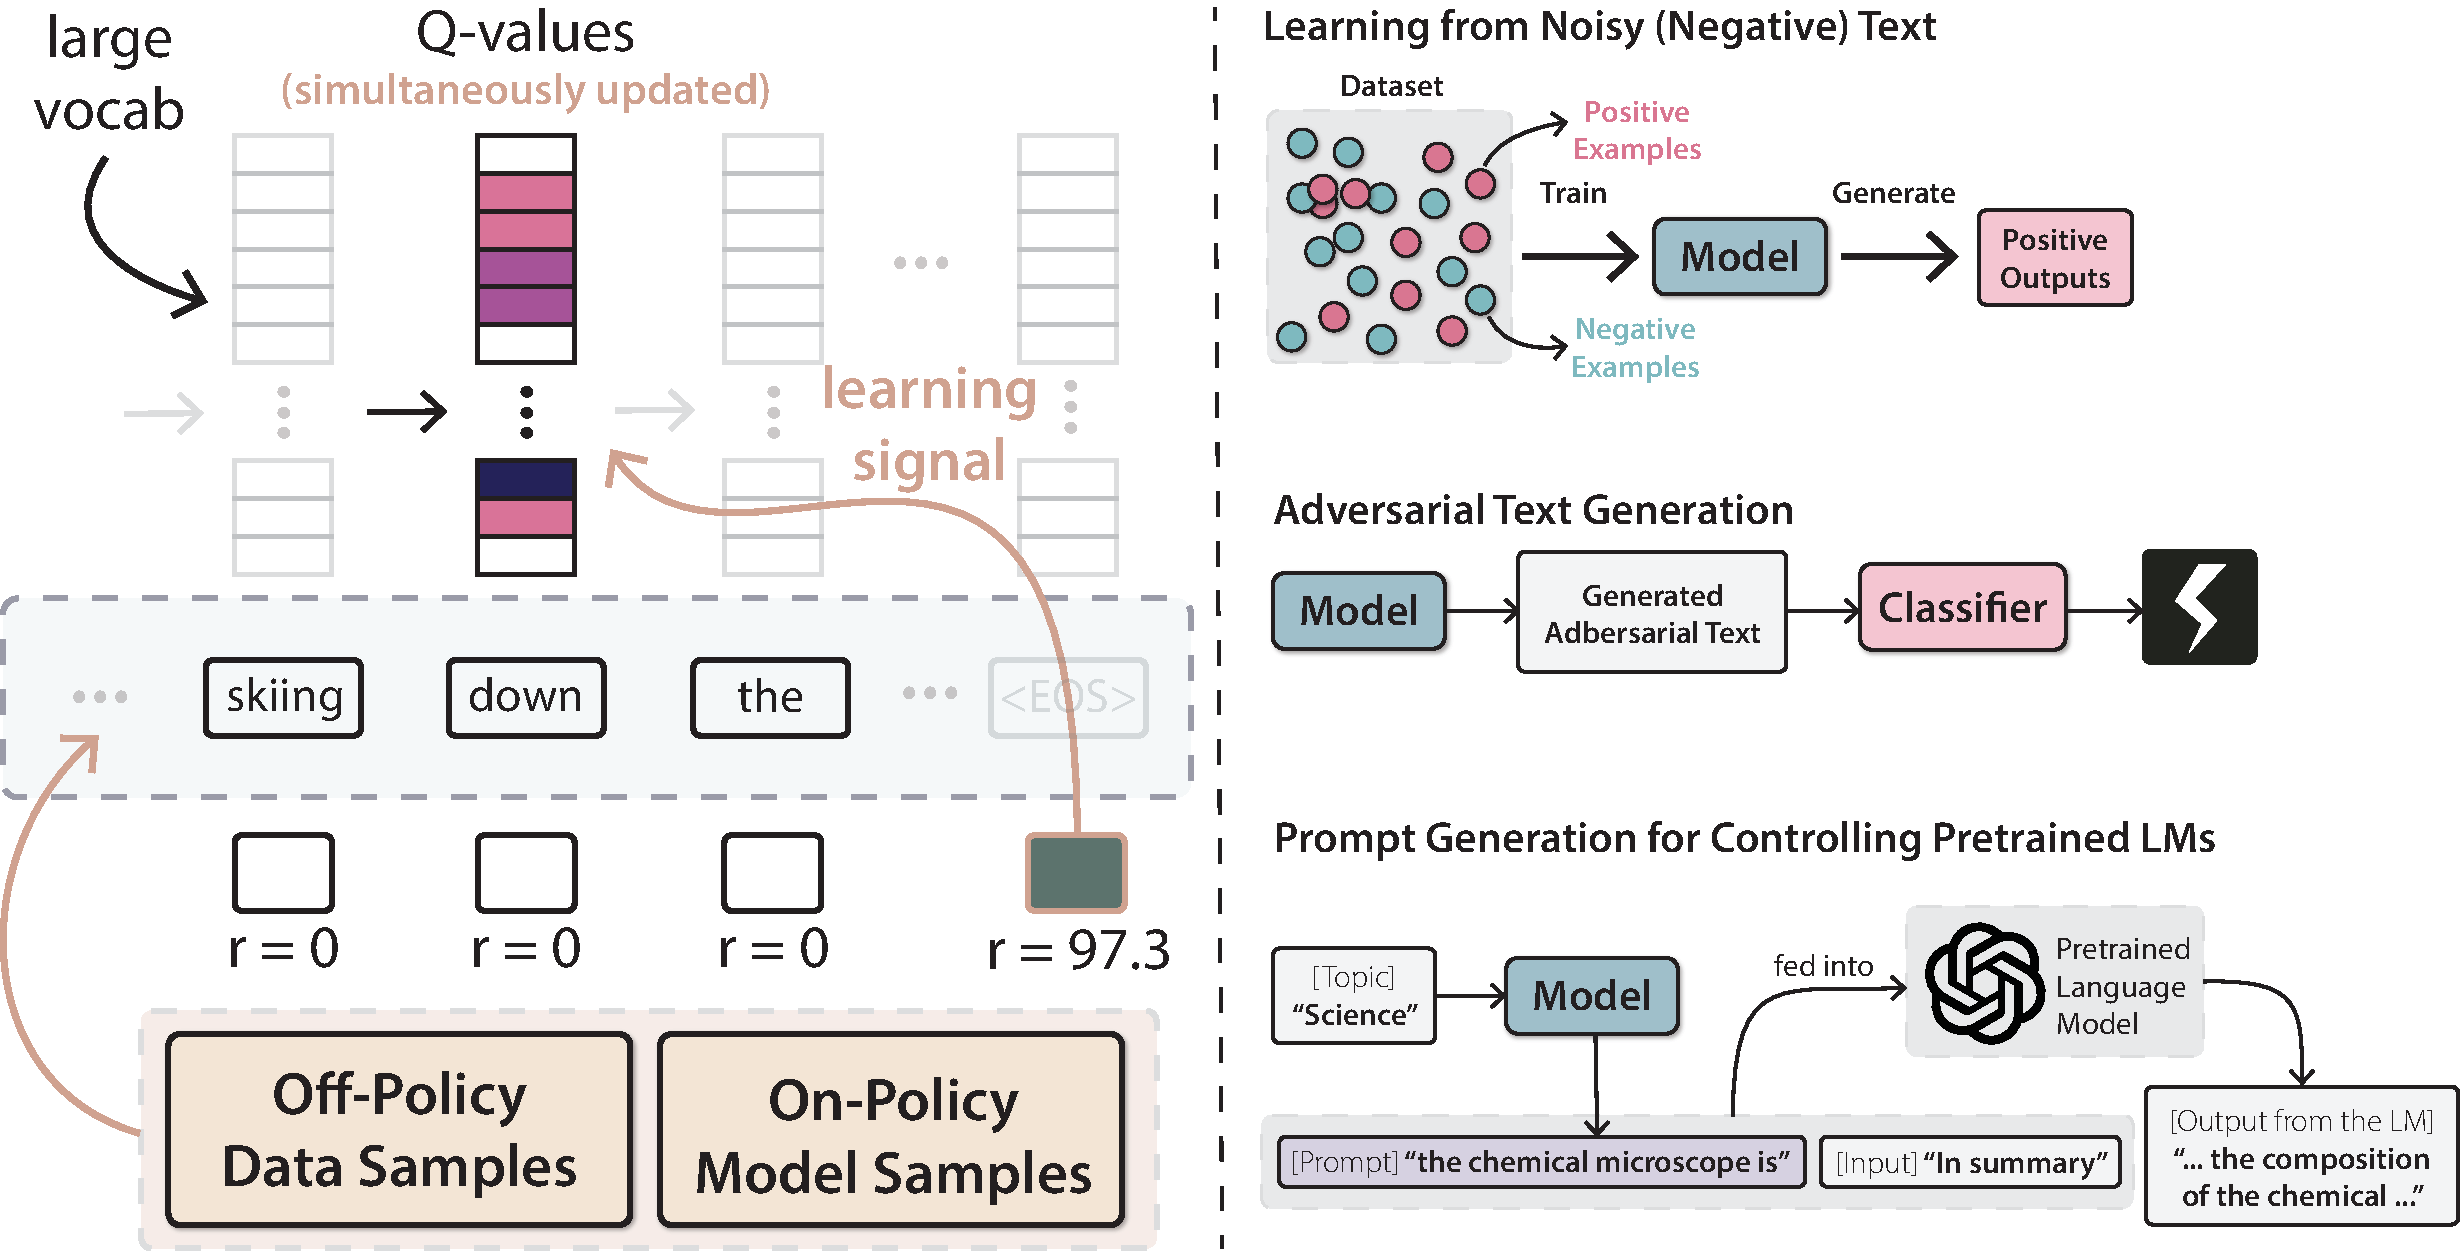
\includegraphics[width=0.99\linewidth]{figures/20211003-figure1.pdf}
    \vspace{-4pt}
    \caption{
    \textbf{Left:} An overview of the proposed SQL algorithm. Text generation is challenging due to sparse reward (i.e., the rewards of all intermediate steps are $0$) and large action space (i.e., large vocabulary).
    Our SQL formulation enables several key algorithmic features as highlighted with \textcolor[HTML]{D0A28F}{\textbf{yellow}} color, including (1) the combined on- and off-policy updates for the best of both, (2) bridging the final non-zero reward to directly supervise the $Q$-value estimation at intermediate steps for learning stability, and (3) simultaneously updating the $Q$-values of all candidate actions for efficiency. 
    \textbf{Right:} We explore diverse applications of the text-generation RL algorithm.
    }
    \label{fig:first-figure}
    \vspace{-7pt}
\end{figure*}


Another set of work has resorted to \emph{off-policy} RL. The key advantage is that samples from other sources, e.g., human-written text, can be used, making them more data efficient than on-policy methods. Previous work has used either importance weighted PG~\citep{pang2021text,zhou2017end,kandasamy2016batch} or $Q$-learning based algorithms~\citep{guo2015generating,jaques2020human,narasimhan2015language}. However, off-policy methods have been considered to be less stable. For example, the $Q$-learning performance relies heavily on how accurate the learned $Q$-function assesses the quality of intermediate subsequences -- a challenging task due to the sparse reward signals.

In this paper, we develop a new RL formulation for text generation that tackles the above issues (Figure~\ref{fig:first-figure}, left). We reframe the text generation problem from the \emph{soft $Q$-learning} perspective originally developed in robotics \citep{haarnoja2017reinforcement,schulman2017equivalence}. The resulting connection allows us to seamlessly take advantage of the latest successful techniques from the RL literature. 
In particular, we introduce and adapt the principled \emph{path consistency learning} \citep{nachum2017bridging} to text generation, that (1) offers a natural way to train the model with both on- and off-policy updates, hence combining the best of the two strategies, (2) bridges the sparse reward signal to directly supervise the $Q$ function learning, leading to more accurate $Q$ estimation and credit assignment, and (3) makes efficient updates to $Q$-values by considering all candidate actions together. 

The generality and efficiency of the proposed method allows us to train text generation in a wide range of applications: (1) With \emph{noisy and negative training examples}, our approach learns to generate accurate entailment text that greatly improves upon the data itself as well as other various training methods; (2) Our approach also manages to train an effective \emph{adversarial text generator} for robustness test for classifiers; (3) We train a \emph{prompt generator} with our algorithm to achieve {controllable generation} of pretrained LMs in terms of topics.\footnote{More recently,~\citet{deng2022rlprompt} extend this line of work to optimize discrete text prompts with reinforcement learning.} On all the three tasks, our approach consistently improves over not only previous RL algorithms for text generation, but also diverse task-specialized methods designed specifically for each of the problems, respectively.
In the appendix (\S\ref{appendix-subsec:standard-tasks}), we also show that on standard supervised tasks where MLE prevails, our approach is competitive to train text generation models \emph{from scratch}, which was usually impossible for previous RL algorithms.







The contributions can be summarized as follows. On the technical side, we propose a new RL formulation for text generation based on soft $Q$-Learning. This new formulation allows us to seamlessly take advantage of the RL literature's latest successful techniques (notably the path consistency algorithm) to overcome the longstanding challenges (e.g., sparse reward and large action space) in text generation.
On the empirical side, we conduct studies on a wide variety of text generation tasks with limited data (i.e., generating from noisy/negative data, adversarial text generation, prompt generation). We propose their RL formulations, and show that our general approach consistently improves over not only previous text RL algorithms, but also diverse task-specialized methods.
